% TODO START

Tähän tulee tietoa kurssin harjoitustehtävien tekemisestä.

% TODO END

\section{Harjoitus 1}

% TODO START

Tavoitteena selvittää jonkin mobiililaitteen ohjelmointiin vaadittavat asiat.

* Valitse laite joka kiinnostaa( esimerkiksi oma puhelin tai tabletti)

* Merkki, mallii?

* Selvitä laitteen käyttöjärjestelmä versio ja ominaisuudet. (Linkki valmistajan esitteeseen?)

* Selvitä mahdolliset ohjelmointi kielet.

* Selvitä ohjelmointiin tarvittavat työkalut ( + käyttöjärjestelmät?)

* Sisältääkö laite valmistajakohtaisia sovelluksia tai ominaisuuksia? Ja mitä tarkoitetaan (mainos)termillä ”puhdas Android”?

* ”App Store” (laitteen / valmistajan) – onko sinne mahdollista saada itsekoodattu sovellus?

* Selvitä laitteesta löytyvät ominaisuudet (esim GPS) ja pystytäänkö niitä käyttämään alustan tarjoamilla ohjelmointikielillä.

Tavoitteena noin sivun mittainen selvitys, jossa viittauksia lähteisiin. Kaikkia tietoja ei
tarvitse kirjata vaan lähteiden viitteitä voi käyttää apuna(esimerkkinä puhelimen
ominaisuuksia ei kannata kaikkia kirjata)

% TODO END

\section{Harjoitus 2}

Versionhallinnan käyttö on tullut aloitettua lähes 10 vuotta sitten ja on
välttämätön työkalua niin töissä, opiskelussa kuin vapaa-ajan projekteissakin,
joten uskon käytön vähintään peruskäytön hallitsevan. Tämän vuoksi erillistä
harjoitus ohjeen mukaista harjoitus2\_vastaus.txt-tiedostoa ei ole lisätty.

Käytössä on lisäksi ssh-avaimet, kuten harjoituksessa viitattiin. Näiden
lisäksi myös commitit allekirjoitetaan ja käytössä submoduuleja. Näistä oli
tarkemmin selitystä aloitus-osiossa.

Oppimispäiväkirja on myös versionhallinnassa ja PDF-muoto siitä generoidaankin
automaattisesti Github Actioneilla, jotka ovat merkittävä apu asioiden
automatisoinnissa kätevästi versionhallinnan kanssa.

\section{Harjoitus 3}

Android Studion asentamisesa on kerrottu tarkemmin aloitus-osiossa.

Oppimispäiväkirja-repository ja sen myötä myös harjoituksien kansiot
sijaisevat WSL:n tiedostojärjestelmässä. Tähän on keino päästä käsiksi kuten
mm. verkkojakoihin, toisiin kovalevyihin yms. Android Studio ei kuitenkaan
toimi tämän kautta vaan näyttää \ref{fig:android-studio-path-not-writable}
mukaisen virheen, ettei kansio ole kirjoitusoikeuksia.

\begin{figure}[h!]
    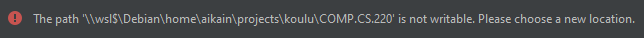
\includegraphics[width=\textwidth]{figures/android-studio-path-not-writable.png}
    \caption{Kuvankaappaus Android Studio virheestä kirjoittaa kansioon}
    \label{fig:android-studio-path-not-writable}
\end{figure}

Projektin voi kuitenkin luoda muutoin WSL:n puolelle ja sen jälkeen avata
Android Studiolla. Tästä kuitenkin aiheutuu uusi ongelma; Gradle ei saa
syncattua haluamiaan asioita vaan sanoo ''virhe, yritä uudelleen'' tarkentamatta
mikä virhe. Logeista löytyy hiukan tarkempi virhe:

\begin{displayquote}
GradleConnectionException: Operation result has not been received
\end{displayquote}

Tämän virheen perusteella ei kuitenkaan löydy mitään Android Studioon itseensä
liittyvää vaan kaikki viittaavat kahteen Intellij IDEAn issueeseen (joka toki
tässä tapauksessa on tarpeeksi lähellä), mutta molemmissa puhutaan Android-
lisäosan kytkemisestä pois päältä ja se ei oikein toimi ratkaisuna tähän
tilanteeseen.

On hyvin mahdollista, että virhe johtuu SDK:n sijaitsemisesta Windowsin
puolella kun kaikki muut (projekti, gradle, jdk) sijaisevat WSL:n sisällä.
Kuitenkin kokemuksen pohjalta yleensä fyysisten laitteiden kanssa kommunikointi
WSL:n sisältä käsin on hyvin nihkeää ja jo emulaattorinkin käyttö saattaisi
tuottaa ongelmia, joten ei ole mielekästä lähteä asentamaan Android SDK:ta ja
kaikkea siihen liittyvää WSL:n sisälle.

Pitkälti siis ainut toimiva ja aikaa säästävä ratkaisu on pitää projektit
Windowsin puolella. Kuitenkaan yksittäisten projektin vuoksi en ole siirtämässä
versionhallintaa ja kaikkea muuta configuraatiota toimimaan WSL:n ulkopuolella,
joten tarvitaan keino pitää repo WSL:ssä, mutta harjoitustehtävät Windowsin
puolella. Ensimmäisenä tähän tulee mielenä yksinkertaisesti käyttää symboolista
linkkiä.

\begin{lstlisting}[
    basicstyle=\small,
    label={lst:symbolic-link-harjoitustehtavat},
    language=bash,
]
    # ln -s /mnt/c/Users/Aikain/AndroidStudioProjects/mobiiliohjelmointi-kurssi-harjoitustehtavat/ harjoitustehtavat
\end{lstlisting}

Symboolin linkki näkyy kuitenkin Gitille symboolisena linkkinä eikä normaaleina
tiedostoina, mikä toki on täysin perusteltua mm. tietoturvasyistä. Puolestaan
ns. kovan linkin tekeminen ei ole mahdollista kansioille. Vaihtoehtoisesti
voisi kokeilla linkin tekemistä toisinpäin
\parencite{StackoverflowWSLSymlink}.

\begin{lstlisting}[
    basicstyle=\small,
    label={lst:powershell-link-harjoitustehtavat},
    language=PowerShell,
]
    New-Item -ItemType SymbolicLink -Path ''C:\Aikain\Users\AndroidStudioProjects\mobiiliohjelmointi-harjoitustehtavat'' -Target ''\\wsl$\Debian\home\aikain\projects\COMP.CS.220\harjoitustehtavat''
\end{lstlisting}

Tämä kuitenkin aiheuttaa jälleen samat ongelmat kuin aiemmin Android Studion
kanssa kun yritti käyttää suoraan WSL:n sisällä olevaa sijaintia.

Ei ehkä niin hyvänä ratkaisuna, mutta kuitenkin toistaiseksi toimiva ratkaisu
saadaan käyttämällä bind mountia \parencite{BaeldungBindMounts}.

\begin{lstlisting}[
    basicstyle=\small,
    label={lst:bind-mount-harjoitustehtavat},
    language=bash,
]
    $ mount -o bind /mnt/c/Users/Aikain/AndroidStudioProjects/mobiiliohjelmointi-harjoitustehtavat /home/aikain/projects/koulu/COMP.CS.220/harjoitustehtavat
\end{lstlisting}

% TODO START

Harjoitus1-3 käytetty 2h 50min

% TODO END
